\documentclass{article}
\usepackage[latin1]{inputenc}
\usepackage[T1]{fontenc}
\usepackage{lmodern}
\usepackage{amsmath}
\usepackage{tkz-tab}

\newcommand*{\va}{\colorbox{red!50}    {$\scriptscriptstyle V_a$}}
\newcommand*{\vb}{\colorbox{blue!50}   {$\scriptscriptstyle V_b$}}
\newcommand*{\vbo}{\colorbox{blue!50}  {$\scriptscriptstyle V_{b1}$}}
\newcommand*{\vbt}{\colorbox{yellow!50}{$\scriptscriptstyle V_{b2}$}}
\newcommand*{\vc}{\colorbox{gray!50}   {$\scriptscriptstyle V_c$}} 
\newcommand*{\vd}{\colorbox{magenta!50}{$\scriptscriptstyle V_d$}} 
\newcommand*{\ve}{\colorbox{orange!50} {$\scriptscriptstyle V_e$}}  

\parindent=0pt
\begin{document}
  
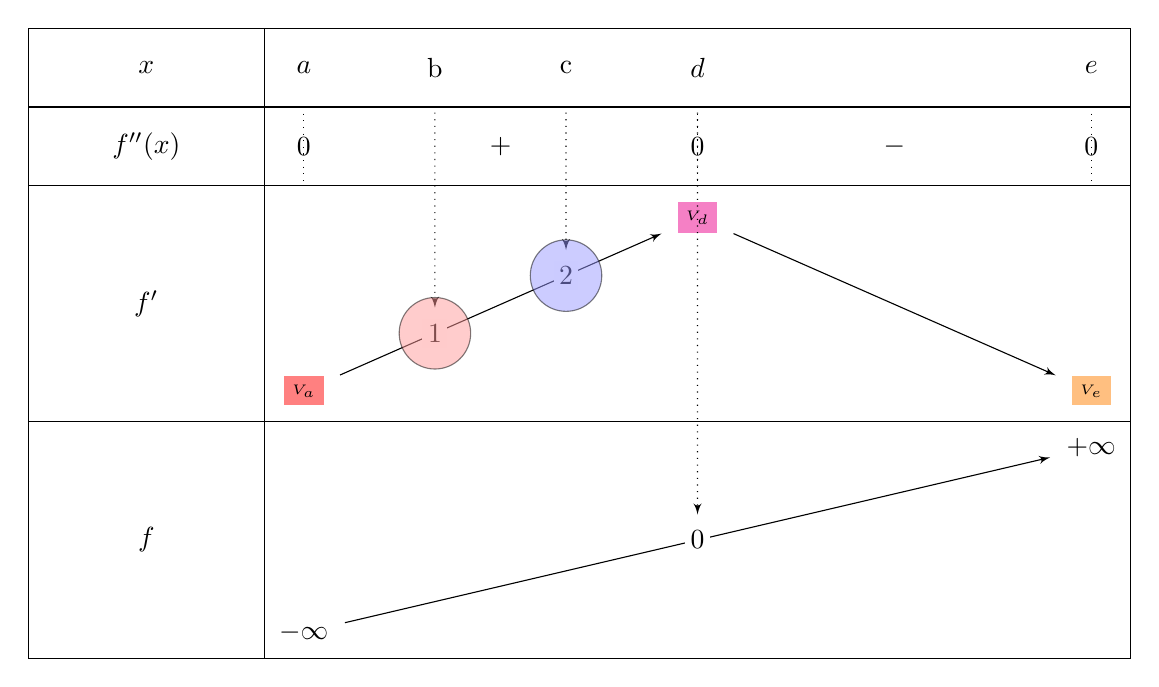
\begin{tikzpicture}
	\tkzTabInit[lgt=3,espcl=5]{ $x$/1,$f''(x)$/1,$f'$/3,$f$/3 }%
	           {  $a$    , $d$    ,$e$}
	\tkzTabLine{  z,+    ,z,-     ,z  } 
	\tkzTabVar  {-/\va  ,+/\vd   , -/  \ve}
	\tkzTabVal[draw,remember=vb]{1}{2}{0.333}{b}{$1$}
	\tkzTabVal[draw,remember=vc]{1}{2}{0.666}{c}{$2$}
	\tkzTabVar{-/$-\infty$  ,R/   , +/  $+\infty$}
	\tkzTabVal[draw]{1}{3}{0.5}{}{$0$}
  \draw[opacity=0.5,fill=red!40]  (vb) circle(3ex);
  \draw[opacity=0.5,fill=blue!40] (vc) circle(3ex);
\end{tikzpicture}
\end{document}

% latin1
% pdflatex
% Alain Matthes